\chapter{Simulación}

La simulación es un proceso que nos permite estudiar el comportamiento de un sistema complejo que es muy difícil de examinar de manera analítica. Nos ayuda a determinar de manera empírica las probabilidades de ciertos eventos. La simulación nos permite experimentar con diversos supuestos que podrían ser muy costosos de realizar. Las áreas en las que se utiliza la simulación como herramienta diaria son por ejemplo en biología, estadística, medicina, química, matemáticas, investigación de operaciones, física, ingeniería o en las ciencias sociales.

Algunos ejemplos de su aplicación van desde simular el lanzamiento de una moneda justa, hasta la simulación de colisiones de átomos en un acelerador de partículas. Se utiliza para todo tipo de propósitos, por ejemplo para poder realizar predicciones en base a datos históricos o enseñar a los pilotos a volar un avión sin poner en riesgo a la población al volar el avión real.

Actualmente se combinan diferentes metodologías de simulación con el software disponible, el análisis de sensibilidad y la optimización estocástica para poder obtener un mejor resultado al momento de simular sistemas que se hacen cada vez más complejos como las redes neuronales.

A lo largo de este capítulo explicaremos el proceso que seguimos para obtener la asignación de los horarios para cada materia con su respectivo profesor.

\section{Funciones hechas en R}

El diagrama de flujo de la función \textbf{gen\_asignacion} se puede ver en la figura \ref{DF_genAsig}.

\begin{figure}[H]
\centering
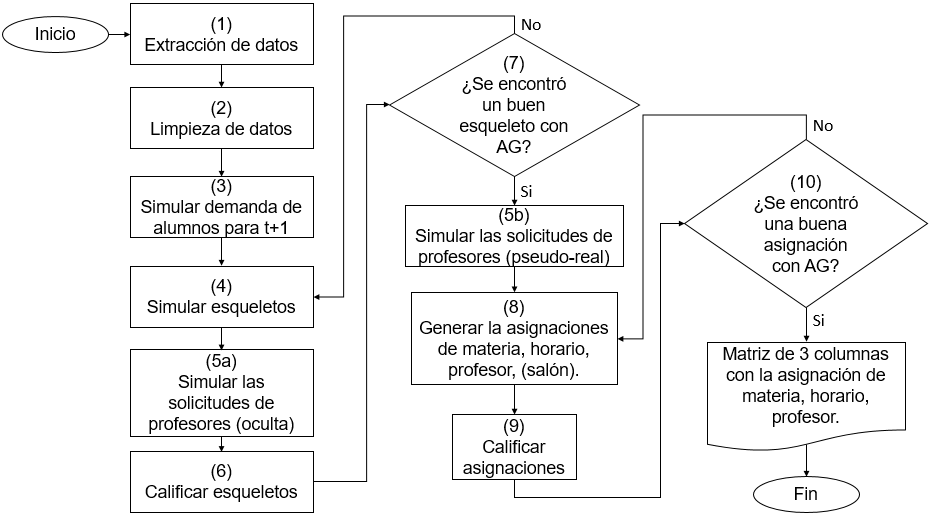
\includegraphics[scale = 0.7]{diagrama_flujo} %width=\textwidth
\caption{\textit{Diagrama de flujo de la función \textbf{gen\_asignacion}}}\label{DF_genAsig}
\end{figure}


\begin{itemize}
\item \textit{posibles\_url}

\item \textit{gen\_m\_grande}

\item \textit{gen\_m\_grande\_total}

\item \textit{gen\_esqueleto: } Función que genera esqueletos la cual carga la función \textit{simula\_grupos} y ésta a su vez carga la función \textit{estima\_grupos}.

\item \textit{gen\_solicitudes}

\item \textit{gen\_asignacion}

\item \textit{gen\_simula\_alumnos}

\item \textit{gen\_simula\_tamano\_grupo}
\end{itemize}

\section{Obtención de los parámetros $q_{1}$ y $q_{2}$}

En esta sección vamos a explicar cómo obtuvimos los valores de $q_{1}$ y $q_{2}$. Son parámetros que se introducen en la función \verb@hw()@ de \textit{R}. Representan los cuantiles utilizados al calcular los intervalos de confianza. Por ejemplo si $q_{1} = 80$ entonces se calcula el intervalo al $80\%$ de confianza. Si se introducen a la función los dos parámetros entonces se calculan dos intervalos, uno al $q_{1}\%$ de confianza y el otro al $q_{2}\%$ de confianza.

Primero definimos los parámetros generales necesarios para las simulaciones:

\begin{enumerate}
\item Fijamos la semilla con \verb@set.seed(8654)@.

\item Elegimos 3 semestres para simular la demanda del número de alumnos. Los seleccionamos de los semestres que ya teníamos guardados con información real. Hicimos una comparación entre nuestros datos simulados y los reales de cada semestre. Los semestres que elegimos fueron: 2019-1, 2019-2 y 2020-1.

\item Fijamos $k = 5$ (número de semestres que se tienen como ventana de información).

\item Fijamos $num\_sim = 10$ (número de simulaciones de la demanda de alumnos para el semestre a simular).
\end{enumerate}


Después fijamos 5 materias que consideramos representativas para hacer las pruebas iniciales: \textit{Cálculo Diferencial e Integral I}, \textit{Demografía I}, \textit{Modelos no Paramétricos y de Regresión}, \textit{Administración de Riesgos Financieros} y \textit{Seminario de Investigación de Operaciones}.

Tomamos 12 posibles combinaciones de valores para $q_{1}$ y $q_{2}$, las cuales podemos ver en la \tablename{\ref{valoresQ1Q2}}. La letra \textit{L} indica que se tomó la cota inferior de $q_{1}$ y la letra \textit{U} indica que se tomó la cota superior de $q_{2}$. Con estas cotas formamos intervalos de los cuales obtuvimos las simulaciones para los 3 diferentes semestres previamente elegidos. %Con las cotas de tipo \textit{$Lq_{1}$,$Uq_{2}$} se forma un intervalo del que s

\begin{table}[H]
\centering
\begin{tabular}{|c|c|c|c|c|}
\hline 
$q_{1} \backslash q_{2}$ & 80 & 85 & 90 & 99 \\ 
\hline 
80 & - & L80,U85 & L80,U90 & L80,U99 \\ 
\hline 
85 & L85,U80 & - & L85,U90 & L85,U99 \\ 
\hline 
90 & L90,U80 & L90,U85 & - & L90,U99 \\ 
\hline 
99 & L99,U80 & L99,U85 & L99,U90 & - \\ 
\hline 
\end{tabular} 
\caption[\textit{Posibles valores para $q_{1}$ y $q_{2}$}]{\textit{Posibles valores para $q_{1}$ y $q_{2}$: Tabla que muestra todas las combinaciones de los intervalos formados con las cotas inferiores y superiores de $q_{1}$ y $q_{2}$}}\label{valoresQ1Q2}
\end{table}


Una vez hecha la simulación obtuvimos una tabla con 7 columnas: materia, intervalo, mín, media, máx, sd y seg. Donde en el renglón i se tienen los datos de la matriz de diferencias relativas de la i-ésima materia para cada intervalo de $q_{1}$ y $q_{2}$. La matriz de diferencias relativas se genera al restar, para cada materia, los datos reales menos los simulados y después dividirlos entre los reales. Por ejemplo en el primer renglón de la \figurename{\ref{matMedDispersion}} vemos que se utilizó el intervalo $(L80,U85)$ para obtener el número de alumnos simulados para el siguiente semestre de la materia \textit{Cálculo Diferencial e Integral I}. Las columnas 2, 3, 4 y 5 corresponden a las medidas de la matriz de diferencias relativas para cada materia. La última columna indica el tiempo que se tardó el proceso.

\begin{figure}[H]
\centering
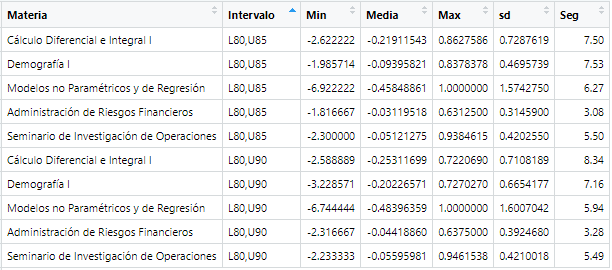
\includegraphics[scale = 0.9]{mat_med_dispersion} %width=\textwidth
\caption[\textit{Matriz con información por materia}]{\textit{Matriz con información por materia: vemos los primeros 10 renglones de la tabla obtenida con información de la matriz de diferencias relativas.}}\label{matMedDispersion}
\end{figure}


Decidimos elegir $q_{1}$ y $q_{2}$ en base a la desviación estándar. Con la \figurename{\ref{matMedDispersion}} obtuvimos una matriz de dos columnas que contine en su primer columna el intervalo y en la segunda el promedio de la desviación estándar para cada intervalo de las 5 materias. Los datos de dicha matriz los podemos ver en la \figurename{\ref{promSD_5m_12p}}.

\begin{figure}[H]
\centering
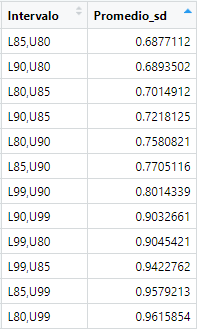
\includegraphics[scale = 1]{prom_SD_5m_12p} %width=\textwidth
\caption[\textit{Promedio de la desviación estándar: 5 materias, 12 pruebas}]{\textit{Promedio de la desviación estándar: 5 materias, 12 pruebas: Matriz con el promedio de la desviación estándar para 5 materias y 12 diferentes intervalos.}}\label{promSD_5m_12p}
\end{figure}


Los datos en la \figurename{\ref{promSD_5m_12p}} están ordenados de menor a mayor con respecto al promedio de la desviación estándar. Para la segunda prueba se eligieron los primeros 6 intervalos de dicha tabla. Se eligieron 10 materias: \textit{Álgebra Lineal I}, \textit{Álgebra Superior II}, \textit{Algoritmos Genéticos}, \textit{Análisis Matemático IV}, \textit{Análisis Numérico}, \textit{Teoría de la Medida I}, \textit{Cálculo Diferencial e Integral IV}, \textit{Graficas y Juegos}, \textit{Inglés I} y \textit{Matemáticas Actuariales para Seguro de Daños}. La tabla con el promedio de la desviación estandar de sus datos se puede ver en la \figurename{\ref{promSD_10m_6p}}.


\begin{figure}[H]
\centering
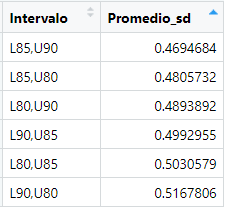
\includegraphics[scale = 1]{prom_SD_10m_6p} %width=\textwidth
\caption[\textit{Promedio de la desviación estándar: 10 materias, 6 pruebas}]{\textit{Promedio de la desviación estándar: 10 materias, 6 pruebas: Matriz con el promedio de la desviación estándar para 10 materias y 6 diferentes intervalos.}}\label{promSD_10m_6p}
\end{figure}


Para la tercera prueba elegimos, de la \figurename{\ref{promSD_10m_6p}} los intervalos que tuvieran un promedio en la desviación estándar menor a $0.5$. Seleccionamos otras 10 materias: \textit{Estadística III}, \textit{Teoría del Seguro}, \textit{Programación Entera}, \textit{Investigación de Operaciones}, \textit{Geometría Moderna I}, \textit{Geometría Analítica II}, \textit{Lógica Matemática I}, \textit{Cálculo Diferencial e Integral III}, \textit{Estadística I} y \textit{Bases de Datos}. La tabla con el promedio de la desviación estandar de sus datos se puede ver en la \figurename{\ref{promSD_10m_4p}}.


\begin{figure}[H]
\centering
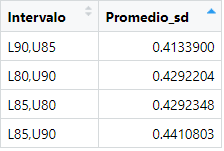
\includegraphics[scale = 1]{prom_SD_10m_4p} %width=\textwidth
\caption[\textit{Promedio de la desviación estándar: 10 materias, 4 pruebas}]{\textit{Promedio de la desviación estándar: 10 materias, 4 pruebas: Matriz con el promedio de la desviación estándar para 10 materias y 4 diferentes intervalos.}}\label{promSD_10m_4p}
\end{figure}

Podemos ver que los valores de la \figurename{\ref{promSD_10m_4p}} son muy parecidos. Hicimos una prueba con los mismos intervalos pero con 5 materias que se dan en todos los semestres y además tienen muchos alumnos. Hicimos la prueba para ver si había alguna diferencia en los datos y poder elegir un sólo intervalo. Las materias que elegimos para esta prueba fueron: \textit{Geometría Analítica I}, \textit{Cálculo Diferencial e Integral II}, \textit{Finanzas I}, \textit{Probabilidad II} y \textit{Procesos Estocásticos I}. La tabla con el promedio de la desviación estandar de sus datos se puede ver en la \figurename{\ref{promSD_5m_4p}}.


\begin{figure}[H]
\centering
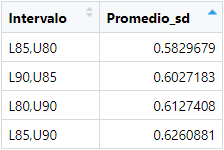
\includegraphics[scale = 1]{prom_SD_5m_4p} %width=\textwidth
\caption[\textit{Promedio de la desviación estándar: 5 materias, 4 pruebas}]{\textit{Promedio de la desviación estándar: 5 materias, 4 pruebas: Matriz con el promedio de la desviación estándar para 5 materias y 4 diferentes intervalos.}}\label{promSD_5m_4p}
\end{figure}

Analizando la información de las matrices de las Figuras \ref{promSD_10m_4p} y \ref{promSD_5m_4p}, decidimos elegir los valores de $q_{1} = 85$ y $q_{2} = 80$. Por lo que el intervalo que buscamos estará formado por la cota inferior del intervalo de confianza al $85\%$ y por la cota superior del intervalo de confianza al $80\%$. Para visualizar de una mejor manera cómo se encuentra el intervalo formado, podemos ver la \figurename{\ref{interConf}}. De ese intervalo vamos a obtener los valores para simular la demanda de alumnos.

\begin{figure}[H]
\centering
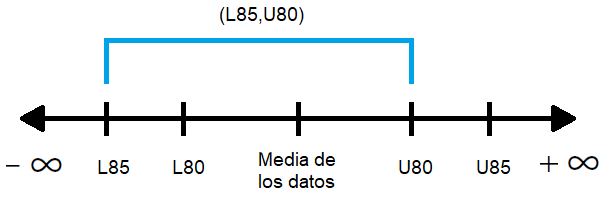
\includegraphics[scale = 0.7]{intervalos_confianza} %width=\textwidth
\caption[\textit{Diagrama de los intervalos de confianza}]{\textit{Diagrama de los intervalos de confianza: Se muestra el intervalo del que se va a obtener el número de alumnos para la simulación de cada materia en cada hora.}}\label{interConf}
\end{figure}

Finalmente con los valores de $q_{1} = 85$ y $q_{2} = 80$ hicimos una prueba aleatoria (eliminando la semilla). Las materias que elegimos para dicha prueba son: \textit{Estadística III}, \textit{Teoría del Seguro}, \textit{Cálculo Diferencial e Integral I}, \textit{Investigación de Operaciones}, \textit{Geometría Moderna I}, \textit{Geometría Analítica II}, \textit{Lógica Matemática I}, \textit{Cálculo Diferencial e Integral III}, \textit{Estadística I}, \textit{Bases de Datos}, \textit{Matemáticas Financieras}, \textit{Cálculo Diferencial e Integral II}, \textit{Probabilidad I}, \textit{Probabilidad II} y \textit{Procesos Estocásticos I}. Los resultados de la prueba aleatoria los podemos ver en la \figurename{\ref{mat_med_dispersion_pruebaAl}}. El promedio de la desviación estándar de todas las materias es $0.48$.%$0.4814898$.

\begin{figure}[H]
\centering
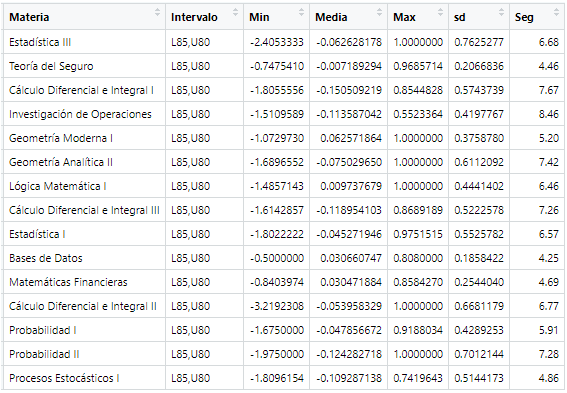
\includegraphics[scale = 0.9]{mat_med_dispersion_pruebaAleatoria} %width=\textwidth
\caption[\textit{Matriz con medidas de dispersión de prueba aleatoria}]{\textit{Matriz con medidas de dispersión de prueba aleatoria: Se muestra en cada renglón la materia y el intervalo del que se tomaron los valores para la simulación.}}\label{mat_med_dispersion_pruebaAl}
\end{figure}
 %%Subsección %%To include subfiles in to a subfiles use \input{name_of_file}

\section{Simulación de la demanda de alumnos}

La demanda del número de alumnos para el siguiente semestre la hicimos por materia y por hora. Para poder hacer la simulación lo primero que hicimos fue acomodar la información que teníamos por semestres y por hora. El procedimiento que seguimos es el siguiente:

\begin{enumerate}
\item Definir el semestre del cual se quiere obtener la simulación.

\item Definir el número de semestres que se quieren como ventana de información.

\item Tomar una submatriz de \textit{m\_grande\_total} con la información de una materia para los semestres en la ventana de información.

\item Para cada semestre dentro de la ventana de información se suma el número de alumnos en cada hora.

\item Se obtiene una matriz de $15 \times k$ ($k$ es el número de semestres en la ventana) como la que se puede ver en la figura \ref{matAl_corregidos}.
\end{enumerate}

%Por ejemplo si teníamos en el semestre 2018-2 una matriz como la que se muestra en la tabla \ref{TablaVariasMaterias} entonces por cada hora sumamos los datos y así para cada semestre.
%\begin{table}[h]
%\centering
%\begin{tabular}{|c|c|c|}
%\hline 
%Horario & Materia 1 & Materia 2 \\ 
%\hline 
%7-8 & 0 & 0 \\ 
%\hline 
%8-9 & 0 & 0 \\ 
%\hline 
%9-10 & 0 & 0 \\ 
%\hline 
%10-11 & 0 & 0 \\ 
%\hline 
%11-12 & 11 & 33 \\ 
%\hline 
%12-13 & 45 & 30 \\ 
%\hline 
%13-14 & 0 & 0 \\ 
%\hline 
%14-15 & 0 & 0 \\ 
%\hline 
%15-16 & 0 & 0 \\ 
%\hline 
%16-17 & 0 & 0 \\ 
%\hline 
%17-18 & 30 & 22 \\ 
%\hline 
%18-19 & 0 & 0 \\ 
%\hline 
%19-20 & 0 & 0 \\ 
%\hline 
%20-21 & 18 & 35 \\ 
%\hline 
%21-22 & 0 & 0 \\ 
%\hline
%\end{tabular} 
%\caption{\textit{Ejemplo de información varias materias}}\label{TablaVariasMaterias}
%\end{table}
%Podemos ver un ejemplo de la matriz que se formó, al aplicar el procedimiento descrito, para varios semestres, en la figura \ref{matAl_corregidos}.

\begin{figure}[H]
\centering
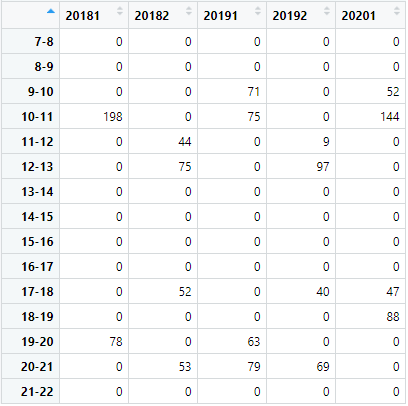
\includegraphics[scale = 0.8]{mat_alumnos_corregidos_EstadisticaIII} %width=\textwidth
\caption{\textit{Ejemplo de matriz con alumnos corregidos}}\label{matAl_corregidos}
\end{figure}

Con el procedimiento descrito pudimos generar vectores por hora y aplicar la función \textit{hw()} en \textit{R} para obtener la demanda de alumnos esperados para el siguiente semestre. En la figura \ref{vec_alum_sim} vemos el vector con la demanda de alumnos simulados para el semestre 2020-2 de la materia \textit{Estadística III}.

Notamos que el valor de la demanda de alumnos es cero cuando en todos los semestres de alguna hora no hay datos. En el ejemplo, es el caso de las 7hrs, 8hrs, 13hrs, 14hrs, 15hrs, 16hrs y 21hrs.

Observando los datos de las 10hrs. vemos que en los semestres pares no hay alumnos, por lo que en la simulación se obtiene únicamente un alumno. Si vemos los datos de las 17hrs vemos que de los 5 semestres en la ventana se tienen alumnos en los semestres pares y en un semestre impar, el número de alumnos simulados para esa hora son 31 alumnos.

Con estos ejemplos podemos ver de manera tangible que el modelo si respeta la estacionalidad semestral que tienen los datos.

\begin{figure}[H]
\centering
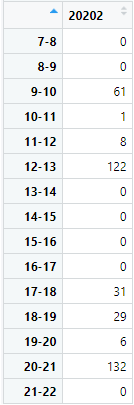
\includegraphics[scale = 0.8]{vec_alum_sim_EstadisticaIII} %width=\textwidth
\caption{\textit{Ejemplo de vector con demanda simulada para el 2020-2}}\label{vec_alum_sim}
\end{figure}

Obtuvimos vectores con la demanda simulada para cada una de las materias y formamos una matriz de $15 \times 333$. En la figura \ref{matDemandaAlum} podemos ver un ejemplo de cómo se ve la matriz formada.

Analicemos 2 pares de grupos, primero veamos la segunda y la quinta columna, que corresponden a las materias de \textit{Álgebra Superior II} y \textit{Geometría Analítica I}, respectivamente. Ambas son materias obligatorias para Actuaría, Matemáticas y Matemáticas Aplicadas. La primera corresponde a semestres pares y la segunda a semestres pares. Notamos que para \textit{Geometría Analítica I}, se tienen alumnos prácticamente en cada hora, pero el número no es muy grande, a diferencia de los alumnos simulados para \textit{Álgebra Superior II}, en donde hay varias horas con cero alumnos simulados pero hay dos grandes cantidades, una a las 9hrs con 832 alumnos y la otra a las 18hrs con 224 alumnos. Con esta comparación podemos ejemplificar la diferencia entre una materia que corresponde a semestres pares con una de semestres impares.

Ahora analicemos las columnas 4 y 8, correspondientes a las materias de \textit{Seminario de Topología A} y \textit{Probabilidad II}. La primera es una materia optativa para Matemáticas y la segunda es una materia obligatoria para Actuaría, correspondiente a semestres pares y optativa para Ciencias de la Computación, Matemáticas y Matemáticas Aplicadas. El número total de alumnos simulados para \textit{Seminario de Topología A} es menor a 20, en cambio para \textit{Probabilidad II} se tiene una gran cantidad de alumnos a las 8hrs, 9hrs y 10hrs. Considerando los valores que se tienen en el turno vespertino para \textit{Probabilidad II}, notamos que a las 19hrs también hay una gran cantidad de alumnos. Con esta comparación podemos ejemplificar la diferencia entre una materia obligatoria y una optativa, así como la diferencia entre el turno matutino y vespertino.


\begin{figure}[H]
\centering
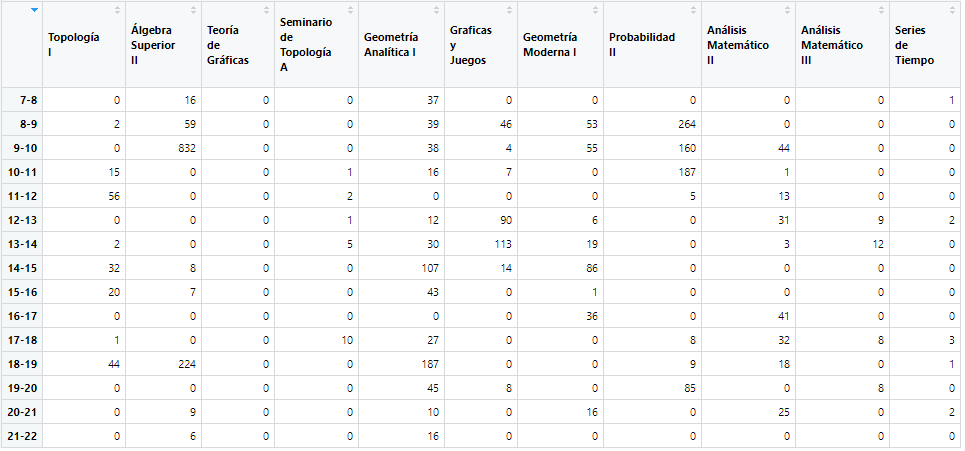
\includegraphics[scale = 0.7]{mat_demanda_alumnos} %width=\textwidth
\caption{\textit{Ejemplo de matriz con demanda simulada para el 2020-2}}\label{matDemandaAlum}
\end{figure}





\section{Simulación de tamaño de grupos}

En esta sección vamos a explicar cómo hicimos la simulación del tamaño de grupos. Vamos a definir al tamaño de un grupo como el número de alumnos que va a tener cada grupo.






\section{Obtención de información para solicitudes}

Antes de iniciar las simulaciones de elección de materia y de horario obtuvimos un vector y una matriz con la información de las materias y de los profesores, respectivamente.

En el caso de las materias, el vector \textit{vec\_nom\_materias\_total} lo obtuvimos a partir de la matriz \textit{m\_grande\_total} del semestre 2008-1 al 2020-1. No tiene nombres repetidos. Tiene 333 materias.

En el caso de los profesores, la matriz \textit{mat\_nom\_prof\_total} tiene 2 columnas. En la primer columna se tienen los nombres de todos los profesores que han impartido clase desde el semestre 2015-1 hasta el 2020-1. Dichos nombres los obtuvimos de la matriz \textit{m\_grande\_total} de los semestres correspondientes.

En la segunda columna de la matriz, se tiene un $1$ si el profesor es de tiempo completo y un $0$ si no. Para llenarla ingresamos a la página \url{http://www.matematicas.unam.mx/index.php/nosotros/profesores-de-tiempo-completo} del Departamento de Matemáticas. Con la aplicación \textit{SelectorGadget} seleccionamos el vector con el nombre de los profesores de tiempo completo. En la figura \ref{profTC_SelectorGadget} podemos ver el código CSS que utilizamos para obtener los datos en R. También observamos que se seleccionaron 94 profesores.

\begin{figure}[H]
\centering
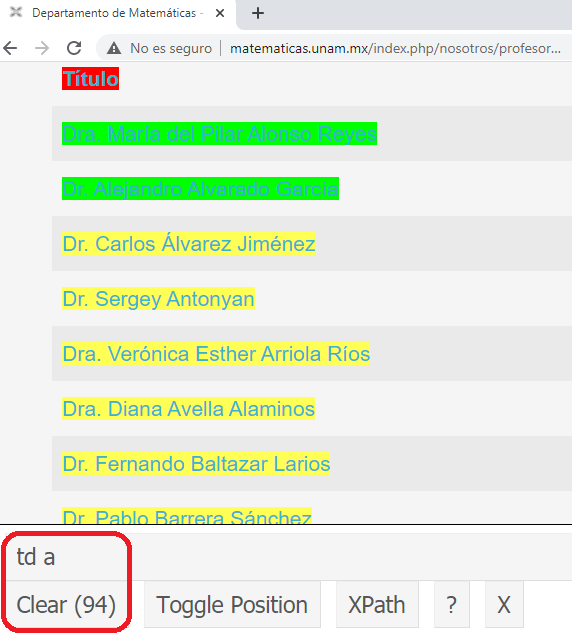
\includegraphics[scale = 0.8]{profesores_TC_SelectorGadget} %width=\textwidth
\caption{\textit{Profesores de tiempo completo: SelectorGadget}}\label{profTC_SelectorGadget}
\end{figure}

Al extraer la información en R obtuvimos un vector con 94 entradas. En la figura \ref{profTC_sinLimpiar} podemos ver los primeros 20 valores del vector. Notamos que cada entrada del vector inicia con los caracteres $\backslash n \backslash t \backslash t \backslash t \backslash t \backslash t \backslash t \backslash t$. Estos caracteres, en la presentación final de la página de internet, indican un salto de línea y las tabulaciones o espacios que se tienen de izquierda a derecha.

\begin{figure}[H]
\centering
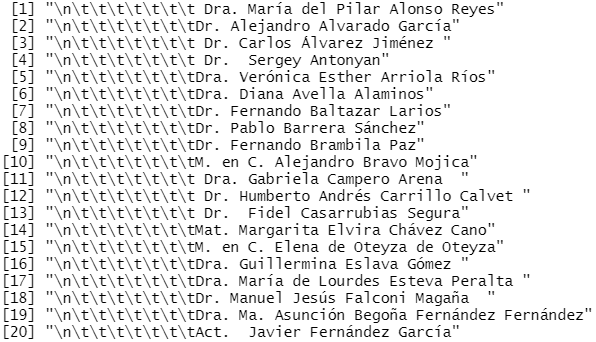
\includegraphics[scale = 0.8]{profesores_TC_sinLimpiar} %width=\textwidth
\caption{\textit{Vector de profesores de tiempo completo}}\label{profTC_sinLimpiar}
\end{figure}

Limpiamos los datos para obtener un vector que sólo tuviera los nombres de los profesores. Eliminamos el título de cada uno porque en los horarios publicados en las páginas de la FC sus nombres no tienen título. También eliminamos los espacios finales que había en algunos nombres.

De esta manera obtuvimos el vector con el nombre de los profesores de tiempo completo del Departamento de Matemáticas. Dicho vector lo comparamos con la primer columna de la matriz \textit{mat\_nom\_prof\_total}, cuando los nombres coincidieron, pusimos un $1$ en el renglón correspondiente.

Al limpiar los datos encontramos 11 nombres que analizamos a mano porque no aparecía el $1$ en su respectivo renglón. Encontramos que no aparecía la información necesaria en la matriz \textit{mat\_nom\_prof\_total} por diferencias en los nombres. Encontramos diferencias por acentos, por mayúsculas y por nombre incompleto. En la tabla \ref{DifNomProfTC} vemos los nombres que aparecen en las páginas de FC comparados con los que aparecen en la página del Departamento de Matemáticas.

\begin{table}[h]
\centering
\resizebox{\textwidth}{!}{%
\begin{tabular}{|c|c|}
\hline 
\textbf{Nombre en páginas de FC} & \textbf{Nombre en página del Depto. de Matemáticas} \\ 
\hline 
Alejandro Ricardo Garciadiego Dantan & Alejandro Ricardo Garciadiego Dantán \\ 
\hline 
Edith Corina Sáenz Valadez & Edith Corina Sáenz Valadéz \\ 
\hline 
Emilio Esteban Lluis Puebla & Emilio Lluis Puebla \\
\hline 
Guillermo Javier Francisco Sienra Loera & Guillermo Sienra Loera \\
\hline 
María Asunción Begoña Fernández Fernández & Ma. Asunción Begoña Fernández Fernández \\ 
\hline 
María Concepción Ana Luisa Solís González-Cosío & Ana Luisa Solís González Cosío \\ 
\hline
María Isabel Puga Espinosa & Isabel Puga Espinosa \\ 
\hline 
María Lourdes Velasco Arreguí & María de Lourdes Velasco Arregui \\ 
\hline 
Mucuy-Kak del Carmen Guevara Aguirre & Mucuy-kak del Carmen Guevara Aguirre \\ 
\hline 
Oscar Alfredo Palmas Velasco & Óscar Alfredo Palmas Velasco \\ 
\hline 
Úrsula Xiomara Iturrarán Viveros & Úrsula Iturrarán Viveros \\ 
\hline 
\end{tabular}
} 
\caption{\textit{Diferencias en nombres de profesores de tiempo completo}}\label{DifNomProfTC}
\end{table}

Finalmente en la matriz \textit{mat\_nom\_prof\_total} se tiene la información de 1387 profesores de los cuales 94 son profesores de tiempo completo.

Algunas notas a considerar de esta matriz son:

\begin{itemize}
\item[-] Hay profesores que se repiten por diferencia de acentos. Ej. \textit{César Alejandro Arellano Ruíz, Luis Eduardo García Hernández}

\item[-] Hay profesores que se repiten por tener a lado el nombre de los ayudantes. Ej. \textit{Fermín Alberto Viniegra Heberlein, Edgar Vázquez Luis}

\item[-] Puede haber profesores que ya no impartan clases en la FC.
\end{itemize}


\section{Simulación de solicitudes de profesores oculta y pseudo-real}

En esta sección vamos a explicar cómo hicimos la simulación de la solicitud de los profesores. En la vida real los profesores pueden elegir libremente las materias que quieren impartir y seleccionan las horas a las que desean impartir sus clases. Dado que no contamos con esa información decidimos simular la elección de materias y horarios en base a la información que tenemos de semestres anteriores.

Como vimos en el diagrama \ref{DF_genAsig} simulamos dos veces las solicitudes de los profesores, en el proceso de asignación. A la primera vez que simulamos las solicitudes la llamaremos \textit{Solicitud oculta} y a la segunda la llamaremos \textit{Solicitud pseudo-real}. La explicación de su uso lo vemos a continuación.

\begin{itemize}
\item[-] Solicitud oculta: La llamamos oculta porque nos ayuda para la generación de los esqueletos. No influye directamente en la asignación final.

\item[-] Solicitud pseudo-real: Es la simulación de las posibles elecciones que los profesores harían en la vida real.
\end{itemize}




\subsection{Simulación de elección de materia}

\subsection{Simulación de elección de horario}



\section{Simulación de esqueletos}

Matriz de 2 columnas (Materia-Horario). En el renglón $i$ se tiene la información de cada grupo simulado para \textit{t+1}.

Se utiliza un matriz auxiliar de 3 columnas (Materia-Horario-Demanda\_Alum). En el renglón $i$ se tiene la información del número de alumnos simulados para la hora y materia correspondientes.

\begin{figure}[H]
\centering
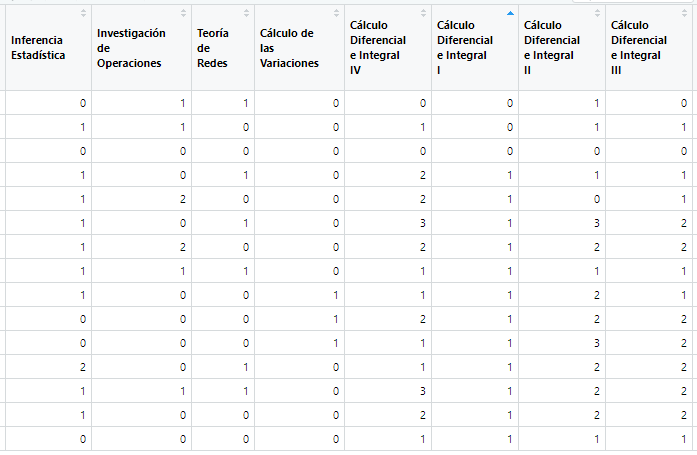
\includegraphics[scale = 0.8]{Ej_esqueleto_20202} %width=\textwidth
\caption{\textit{Ejemplo de esqueleto para el semestre 2020-2}}\label{esqueleto20202}
\end{figure}

\section{Calificación de esqueletos de horario}

\begin{eqnarray*}
L_{materia} &=& -1 \,\,\,\,\,\,  \text{por cada materia no impartida}\\
x &=& \text{promedio}\\
y &=& \text{cupo}\\
L_{dif\_p\_c} (x,y) &=& \begin{cases}
    \dfrac{a}{190} (x-y)  & \quad \text{si } x<y\\
    - \dfrac{b}{190} (x-y)  & \quad \text{si } x\geqslant y
  \end{cases}\\
a &=& 0.5\\
b &=& 0.8\\
L_{categoria}^{1} (mat,solicitud) &=& -c(categoria - 1)\\
L_{categoria}^{2} (mat,solicitud) &=& -c_{1}(categoria)
\end{eqnarray*}

Al momento de simular las solicitudes de materias para los profesores suponemos que la que está en primer lugar es la materia que más quiere dar, en segundo lugar, la segunda que quiere dar.

Primero asignar grupos a los profesores de tiempo completo. Después asignar grupos faltantes a los profesores de asignatura.

$L_{materia}$ es la penalización por no tener en el esqueleto una materia que necesitamos.

$L_{dif\_p\_c}$ es la penalización en la asignación de salones. Se tiene un grupo de tamaño $x$ y un salón con capacidad $y$. Se penaliza con $\dfrac{a}{190}$ veces la diferencia entre $x$ y $y$ cuando el tamaño del grupo es menor a la capacidad del salón y se penaliza con $-\dfrac{b}{190}$ veces la diferencia entre $x$ y $y$ cuando el tamaño del grupo es mayor a la capacidad del salón.

El esqueleto depende de la demanda de alumnos y de las solicitudes de los profesores.

Primero se asignan materias a los profesores de tiempo completo y después a los de asignatura.

Los profesores de asignatura pueden quedarse sin materias asignadas.

Penalizaciones:

\begin{enumerate}
\item Si algún profesor pidió alguna materia y no se la dieron.

\item Si hay alumnos que necesitan una clase a alguna hora y no existe profesor que la imparta.

\item Con $\alpha \times num\_alumnos\_faltantes$ por cada alumno que te faltó en cada hora-materia que tenías que dar. $\alpha > 0$

\item Con $\beta \times num\_alumnos\_sobrantes$ por cada alumno que te pasaste en cada hora-materia que tenías que dar. $\beta > 0$

\end{enumerate}

Queremos el esqueleto con el menor valor en $\alpha + \beta$

Con esto se obtiene un nuevo esqueleto.


\section{Generación de asignaciones}

Matriz de 3 columnas (Materia-Horario-Profesor), la cual tiene la información de las asignaciones. A cada renglón de la matriz de esqueletos se agrega un profesor. Se genera con el esqueleto obtenido del proceso del AG y de las solicitudes de los profesores.

\subsection{Calificación de asignaciones de grupo}

%Los valores del modelo se muestran a continuación:

%\begin{lstlisting}[language=R, caption= \textit{Método Holt-Winters aditivo}]
%Holt-Winters' additive method 
%
%Call:
% hw(y = tsData, h = 1, seasonal = "additive", level = c(q1, q2)) 
%
%  Smoothing parameters:
%    alpha = 0.1247 
%    beta  = 1 
%    gamma = 1 
%
%  Initial states:
%    l = 111 
%    b = -22.5 
%    s = -50 50
%
%  sigma:  155.8648
%\end{lstlisting}

%\begin{figure}[H]
%\centering
%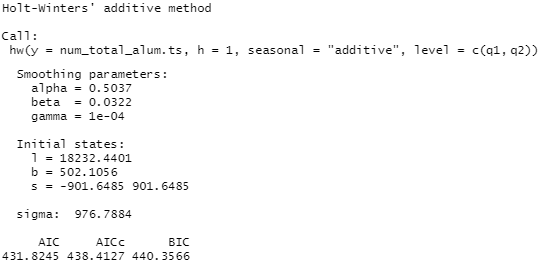
\includegraphics[scale = 0.8]{modelo_HW_total_alumnos_x_sem} %width=\textwidth
%\caption{\textit{Modelo del método aditivo de Holt-Winters: Total de alumnos por semestre}}
%\end{figure}




